% Copyright (c) 2026 CorrectBrain
% SPDX-License-Identifier: MIT

\PassOptionsToPackage{dvipsnames,svgnames,x11names}{xcolor}
\documentclass[tikz,border=8pt]{standalone}
\usetikzlibrary{arrows.meta,positioning,calc,shapes,shadows,decorations.pathmorphing,shapes.geometric,backgrounds,decorations.markings,decorations.pathreplacing,decorations.text,fit,shapes.misc,shapes.arrows,matrix,bending,3d,chains,intersections,shapes.symbols,svg.path,shapes.multipart,snakes,shapes.callouts,angles,quotes,fadings,shadows.blur,patterns,patterns.meta}

\usepackage{amsmath}
\usepackage{amssymb}
\usepackage{fontawesome5}
\usepackage{helvet}
\renewcommand{\familydefault}{\sfdefault}
\usepackage{xcolor}

\providecolor{gold}{RGB}{212,175,55}
\providecolor{silver}{RGB}{192,192,192}
\providecolor{bronze}{RGB}{205,127,50}
\providecolor{darkblue}{RGB}{0,0,139}
\providecolor{lightblue}{RGB}{173,216,230}
\providecolor{darkgreen}{RGB}{0,100,0}
\providecolor{lightgreen}{RGB}{144,238,144}
\providecolor{darkred}{RGB}{139,0,0}
\providecolor{navy}{RGB}{0,0,128}
\providecolor{skyblue}{RGB}{135,206,235}
\providecolor{beige}{RGB}{245,245,220}
\providecolor{cream}{RGB}{255,253,208}

% --- CUSTOM COLOR PALETTE ---
\definecolor{imgblue}{RGB}{52, 152, 219}
\definecolor{imgdark}{RGB}{24, 43, 73}
\definecolor{imgorange}{RGB}{230, 126, 34}
\definecolor{bgcode}{RGB}{30, 30, 30}
\definecolor{bgtitlebar}{RGB}{45, 45, 48}
\definecolor{codeblue}{RGB}{86, 156, 214}
\definecolor{codecyan}{RGB}{156, 220, 254}
\definecolor{codestring}{RGB}{206, 145, 120}
\definecolor{btnred}{RGB}{255, 95, 86}
\definecolor{btnyellow}{RGB}{255, 189, 46}
\definecolor{btngreen}{RGB}{39, 201, 63}

\begin{document}
\begin{tikzpicture}

% --- EXPLICIT STATIC WHITE BACKGROUND ---
\fill[white] (-13, -5) rectangle (13, 15);

% --- TITLE SECTION ---
\node[font=\Huge\bfseries, text=imgdark] at (0.2151,14.5107) {What is a \texttt{w} Descriptor?};
\node[font=\Large, text=imgdark!70, text width=14cm, align=center] at (0, 12.8) {It simply documents the exact native width of the image asset in pixels. It is \textbf{not} a CSS layout width. It is \textbf{not} a display command. It is pure data.};

% --- THE WIDTH RULER ---
\draw[{Bar[width=6mm]}-{Bar[width=6mm]}, line width=2.5pt, imgorange] (-5, 10.5) -- (5, 10.5);
\node[font=\Large\bfseries, text=imgorange, fill=white, inner sep=4pt, anchor=center] at (0, 11.0) {Exactly 1200 physical pixels wide};

% --- THE IMAGE ASSET WINDOW ---
% Frame with smooth blur shadow
\filldraw[fill=white, draw=imgdark!25, line width=1.2pt, rounded corners=8pt, blur shadow={shadow opacity=20, shadow blur radius=4pt}] (-5, 4.0) rectangle (5, 8.0);

% Scenery with realistic gradients and physical pixel grid
\begin{scope}
    \clip[rounded corners=8pt] (-5, 4.0) rectangle (5, 8.0);

    % Sky gradient
    \shade[top color=imgblue!60, bottom color=white] (-5, 4.0) rectangle (5, 8.0);

    % Glowing Sun (concentric fading layers)
    \fill[orange, opacity=0.25] (2.2, 6.6) circle (1.2);
    \fill[yellow!80!orange, opacity=0.45] (2.2, 6.6) circle (0.8);
    \fill[yellow!30!white, opacity=0.90] (2.2, 6.6) circle (0.45);

    % Mountains with depth shading
    \shade[left color=imgblue!80!black, right color=imgblue!40] (-5.5, 4.0) -- (-2.5, 6.6) -- (0, 5.0) -- (2.8, 6.8) -- (5.5, 4.0) -- cycle;
    \shade[left color=imgblue!90!black, right color=imgblue!50] (-3.5, 4.0) -- (-0.8, 5.8) -- (1.2, 4.6) -- (3.8, 6.0) -- (5.5, 4.0) -- cycle;
    \shade[left color=imgdark!95!black, right color=imgblue!70!black] (-5.5, 4.0) -- (-4.0, 5.0) -- (-2.0, 4.0) -- (0.5, 5.2) -- (3.0, 4.0) -- (5.5, 4.8) -- (5.5, 4.0) -- cycle;

    % Pixel Grid Overlay (representing physical pixels)
    \draw[white, opacity=0.3, step=0.2] (-5, 4.0) grid (5, 8.0);
\end{scope}

% Crisp window border overlay
\draw[draw=imgdark!30, line width=1.2pt, rounded corners=8pt] (-5, 4.0) rectangle (5, 8.0);

% Filename Tag positioned on the top-left outer edge of the image frame
\node[font=\large\bfseries, text=imgdark, fill=white, draw=imgdark!15, line width=0.8pt, rounded corners=6pt, inner sep=5pt, blur shadow={shadow opacity=15, shadow blur radius=2pt}, anchor=south west] at (-5, 8.0) {\faFileImage\ hero-large.jpg};

% --- EXPLANATORY NOTE BOX ---
\node[font=\large, text=imgdark, text width=3.5cm, align=center, fill=white, draw=imgorange!40, line width=1.2pt, rounded corners=8pt, blur shadow={shadow opacity=20, shadow blur radius=4pt}, inner sep=10pt, anchor=north west] at (-10, 8.0) {
    {\color{imgorange}\Large\faServer}\\[6pt]
    \textbf{The Core Concept:}\\[4pt]
    The \texttt{w} maps directly to the actual pixel width of the file saved on the server.
};

% --- THE IDE WINDOW ---
% Outer IDE window with shadow
\filldraw[fill=bgcode, draw=gray!40, line width=1pt, rounded corners=8pt, blur shadow={shadow opacity=20, shadow blur radius=4pt}] (-10, -1.5) rectangle (10, 2.5);

% Title Bar with macOS control buttons
\begin{scope}
    \clip[rounded corners=8pt] (-10, -1.5) rectangle (10, 2.5);
    \fill[bgtitlebar] (-10, 1.9) rectangle (10, 2.5);
    \draw[draw=gray!30, line width=0.6pt] (-10, 1.9) -- (10, 1.9);

    % Window control circles
    \fill[btnred] (-9.5, 2.2) circle (0.13);
    \fill[btnyellow] (-9.1, 2.2) circle (0.13);
    \fill[btngreen] (-8.7, 2.2) circle (0.13);
\end{scope}

% Crisp border overlay for IDE window
\draw[draw=gray!40, line width=1pt, rounded corners=8pt] (-10, -1.5) rectangle (10, 2.5);

% Code snippet with precise syntax highlighting using contiguous inline nodes
\node[font=\Large\ttfamily, text=codeblue, inner sep=0pt] (code1) at (-5.6, 0.5) {<};
\node[font=\Large\ttfamily\bfseries, text=codeblue, inner sep=0pt, right=0pt of code1] (code2) {img};
\node[font=\Large\ttfamily, text=white, inner sep=0pt, right=0pt of code2] (code3) {\ };
\node[font=\Large\ttfamily, text=codecyan, inner sep=0pt, right=0pt of code3] (code4) {srcset};
\node[font=\Large\ttfamily, text=gray!80, inner sep=0pt, right=0pt of code4] (code5) {=};
\node[font=\Large\ttfamily, text=codestring, inner sep=0pt, right=0pt of code5] (code6) {"hero-large.jpg\ };
\node[font=\Large\ttfamily\bfseries, text=imgorange, inner sep=0pt, right=0pt of code6] (codew) {1200w};
\node[font=\Large\ttfamily, text=codestring, inner sep=0pt, right=0pt of codew] (code7) {"};
\node[font=\Large\ttfamily, text=white, inner sep=0pt, right=0pt of code7] (code8) {\ };
\node[font=\Large\ttfamily, text=codeblue, inner sep=0pt, right=0pt of code8] (code9) {/>};

% --- THE ZERO-OVERLAP CONNECTOR ARROW ---
% Routed cleanly around obstacles from 1200w bottom anchor directly to the ruler edge
\draw[-Stealth, line width=2pt, imgorange, dashed, rounded corners=15pt]
    (codew.south) -- (codew.south |- 0, -3.0) -- (11.5, -3.0) -- (11.5, 10.5) -- (5.2, 10.5);

\end{tikzpicture}
\end{document}
